\documentclass[aspectratio=169]{beamer}
\usetheme[faculty=phil]{fibeamer}
\usepackage{polyglossia}
\setmainlanguage{english} %% main locale instead of `english`, you
%% can typeset the presentation in either Czech or Slovak,
%% respectively.
\setotherlanguages{russian} %% The additional keys allow
%%
%%   \begin{otherlanguage}{czech}   ... \end{otherlanguage}
%%   \begin{otherlanguage}{slovak}  ... \end{otherlanguage}
%%
%% These macros specify information about the presentation
\title[AGLA2]{Analytical Geometry and Linear Algebra II, Lab 2} %% that will be typeset on the
\subtitle{Gaussian elimination recap\\
          A=LU, A=LDV, PA=LU factorization} %% title page.
\author{Oleg Bulichev}
%% These additional packages are used within the document:
\usepackage{ragged2e}  % `\justifying` text
\usepackage{booktabs}  % Tables
\usepackage{tabularx}
\usepackage{tikz}      % Diagrams
\usetikzlibrary{calc, shapes, backgrounds}
\usepackage{amsmath, amssymb}
\usepackage{url}       % `\url`s
\usepackage{listings}  % Code listings
% \usepackage{subfigure}
\usepackage{floatrow}
\usepackage{subcaption}
\usepackage{mathtools}
\usepackage{todonotes}
\usepackage{fontspec}
\usepackage{multicol}
\graphicspath{{resources/}}
\frenchspacing

\setbeamertemplate{caption}[numbered]
\usetikzlibrary{graphs}

% \usepackage[backend=biber,style=ieee,autocite=footnote]{biblatex}
% \addbibresource{biblio.bib}
% \DefineBibliographyStrings{english}{%
%   bibliography = {References},}

\newcommand{\oleg}[2][] {\todo[color=red, #1] {OLEG:\\ #2}}
\newcommand{\fbckg}[1]{\usebackgroundtemplate{\includegraphics[width=\paperwidth]{#1}}}%frame background

\usepackage[framemethod=TikZ]{mdframed}
\newcommand{\dbox}[1]{
\begin{mdframed}[roundcorner=3pt, backgroundcolor=yellow, linewidth=0]
\vspace{1mm}
{#1}
\vspace{1mm}
\end{mdframed}
}

\begin{document}
\fbckg{fibeamer/figs/title_page.png}
\frame[c]{\setcounter{framenumber}{0}
    \usebeamerfont{title}%
    \usebeamercolor[fg]{title}%
    \begin{minipage}[b][6.5\baselineskip][b]{\textwidth}%
        \textcolor{black}{\raggedright\inserttitle}
    \end{minipage}
    % \vskip-1.5\baselineskip

    \usebeamerfont{subtitle}%
    \usebeamercolor[fg]{framesubtitle}%
    \begin{minipage}[b][3\baselineskip][b]{\textwidth}
        \raggedright%
        \insertsubtitle%
    \end{minipage}
    \vskip.25\baselineskip
}
%   \frame[c]{\maketitle}

\fbckg{fibeamer/figs/common.png}


% \section{Introduction}
% \begin{frame}[t]{\insertsectionhead}

\begin{frame}[c]{Disclaimer regarded to online classes}
\framesubtitle{}

\Large
\begin{block}{How to work with slides}
    \centering I am giving the lecture-like class and answer on questions. All tasks you have to solve by your own at home.
\end{block}
    
\end{frame}

\begin{frame}[t]{Gaussian elimination}
    \framesubtitle{Algorithm}
    \Large
    \begin{equation*}
        \begin{bmatrix}
            2  & 1  & 1 \\
            4  & -6 & 0 \\
            -2 & 7  & 2
        \end{bmatrix}
        \uncover<2>{\rightarrow \alert{\begin{bmatrix}
                    2 & 1  & 1  \\
                    0 & -8 & -2 \\
                    0 & 0  & 1
                \end{bmatrix}}}
    \end{equation*}
\end{frame}

\begin{frame}[t]{Gaussian elimination}
    \framesubtitle{Training task}
    \begin{equation*}
        \left\{\begin{matrix*}[l]
            2x_1+3x_2-x3=9\\
            x_1-2x_2+x_3=3\\
            x_1+2x_3=2
        \end{matrix*}\right.
        \uncover<2->{\alert{\text{Ans: } \left\{\begin{matrix*}[l]
                    x_1=4\\
                    x_2=0\\
                    x_3=-1
                \end{matrix*}\right.}}
    \end{equation*}
\end{frame}


\begin{frame}{A=LU factorization}
    \framesubtitle{Example of A=LU}
    \framesubtitle<3>{Example of A=LDV}
    \Large
    \begin{equation*}
        \underbrace{\begin{bmatrix}
                2  & 1  & 1 \\
                4  & -6 & 0 \\
                -2 & 7  & 2
            \end{bmatrix}}_{A}
        \alert{\uncover<2->{\rightarrow \underbrace{\begin{bmatrix}
                    1  & 0  & 0 \\
                    2  & 1  & 0 \\
                    -1 & -1 & 1
                \end{bmatrix}}_{L}} \only<2>{\underbrace{\begin{bmatrix}
                    2 & 1  & 1  \\
                    0 & -8 & -2 \\
                    0 & 0  & 1
                \end{bmatrix}}_{U}}\uncover<3->{\underbrace{\begin{bmatrix}
                2 & 0  & 0 \\
                0 & -8 & 0 \\
                0 & 0  & 5
            \end{bmatrix}}_{D}\underbrace{\begin{bmatrix}
                1 & 1/2 & 1/2 \\
                0 & 1   & 1/4 \\
                0 & 0   & 1
            \end{bmatrix}}_{\text{$V$ or $U$}}}}
    \end{equation*}
\end{frame}

\begin{frame}[c]{A=LU factorization}
    \framesubtitle{Application: Theory}
    \Large
    \begin{equation*}
        Ax=b \rightarrow \uncover<2->{\underbrace{LU}_{A}x=b}\uncover<3->{ \rightarrow L\underbrace{c}_{Ux}=b}\uncover<4->{\rightarrow Ux=c \rightarrow \alert{\text{Ans: }x}}
    \end{equation*}
    \uncover<4->{There are two steps:
        \begin{enumerate}
            \item \textbf{Factor} (from $A$ find its factors $L$ and $U$)
            \item \textbf{Solve} (from $L$ and $U$ and $b$ find the solution $x$)
        \end{enumerate}
    }
\end{frame}

\begin{frame}[t]{A=LU factorization}
    \framesubtitle{Application: Case Study}
    \vspace{-0.6cm}
    \begin{columns}[T,onlytextwidth]
        \begin{column}{0.49\textwidth}
            \begin{block}{Description}
                Try to solve such systems using:
                \begin{itemize}
                    \item Gauss-Jordan elimination
                    \item LU factorization
                \end{itemize}
                Compare time consuption
            \end{block}
        \end{column}
        \begin{column}{0.49\textwidth}
            \begin{eqnarray*}
                AX=B \text{, where } A = \begin{bmatrix}
                    1  & 2  & 1 \\
                    2  & 3  & 3 \\
                    -3 & 10 & 2
                \end{bmatrix}, B = \begin{bmatrix}
                    k_1 \\k_2\\k_3
                \end{bmatrix} \\
                B_{j+1} = B_j + X_j \text{, for $j=1,2$, where }B_1= \begin{bmatrix}
                    1 \\1\\1
                \end{bmatrix}
            \end{eqnarray*}
        \end{column}
    \end{columns}
    \vspace{-0.8cm}
    \uncover<2->{\small\alert{\begin{equation*}
                A = \overbrace{\underbrace{\begin{bmatrix}
                            \frac{-1}{3} & \frac{16}{29} & 1 \\
                            \frac{-2}{3} & 0             & 0 \\
                            1            & 0             & 0
                        \end{bmatrix}}_{L}\underbrace{\begin{bmatrix}
                            -3 & 10           & 2             \\
                            0  & \frac{29}{3} & \frac{13}{3}  \\
                            0  & 0            & \frac{-21}{2}
                        \end{bmatrix}}_{U}}^{Matlab}=\underbrace{\begin{bmatrix}
                        1  & 0   & 0 \\
                        2  & 1   & 0 \\
                        -3 & -16 & 1
                    \end{bmatrix}}_{L}\underbrace{\begin{bmatrix}
                        1 & 2  & 1  \\
                        0 & -1 & 1  \\
                        0 & 0  & 21
                    \end{bmatrix}}_{U},B_2=\begin{bmatrix}
                    \frac{5}{7} \\ \frac{3}{7} \\ \frac{-4}{7}
                \end{bmatrix},B_3=\begin{bmatrix}
                    \frac{73}{49} \\ \frac{109}{147} \\
                    \frac{-185}{147}
                \end{bmatrix}
            \end{equation*}}}
\end{frame}

\begin{frame}[t]{Task 1}
    \framesubtitle{}
    \begin{figure}[H]
        \centering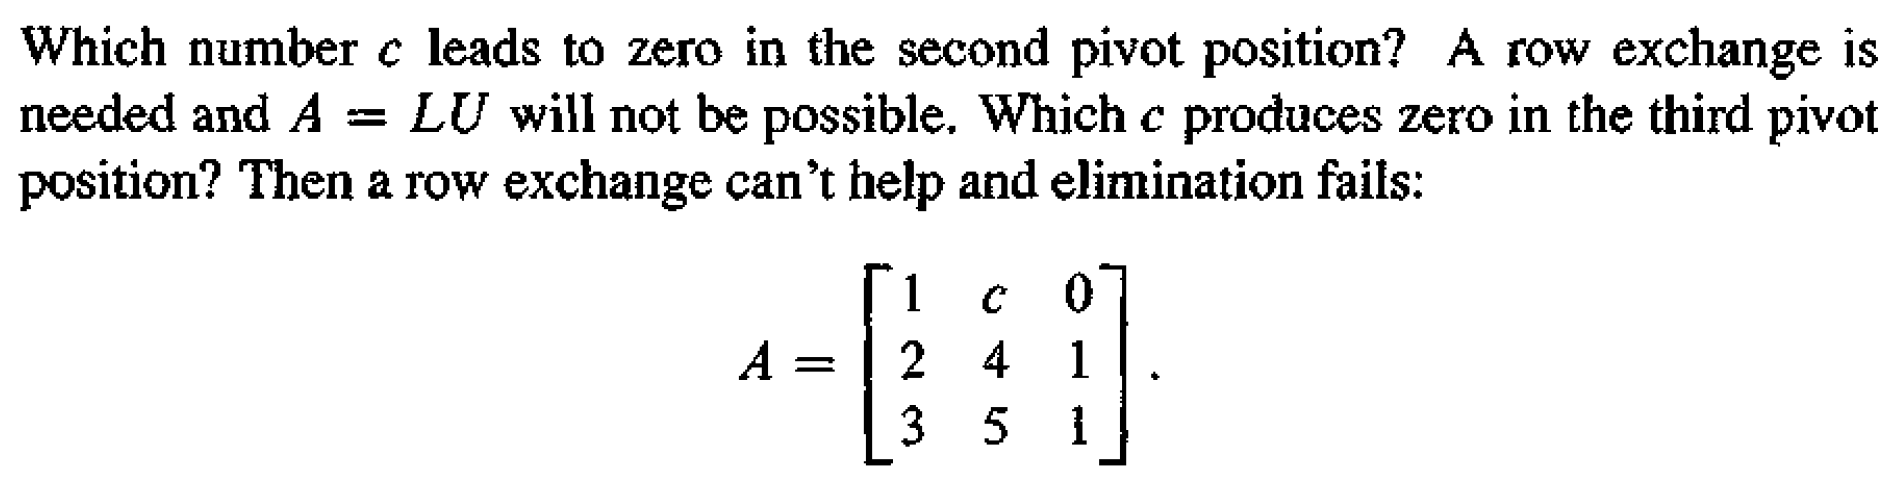
\includegraphics[height=3cm,width=1\textwidth,keepaspectratio]{1.png}
        % \caption{caption_name}
        \label{fig:1.png}
    \end{figure}
    \uncover<2->{
        \alert{\Large Answer}
        \begin{figure}[H]
            \centering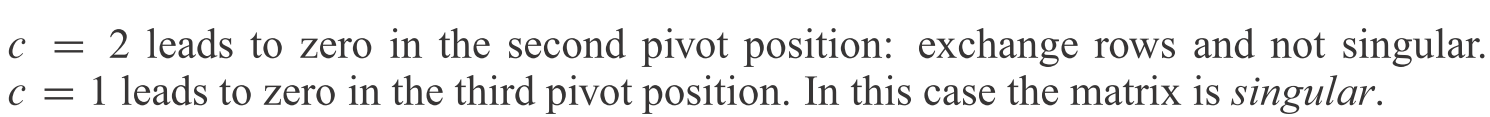
\includegraphics[height=3cm,width=1\textwidth,keepaspectratio]{1ans.png}
            % \caption{caption_name}
            \label{fig:1ans.png}
        \end{figure}
    }
\end{frame}

\begin{frame}[t]{Task 2}
    \framesubtitle{}
    \begin{figure}[H]
        \centering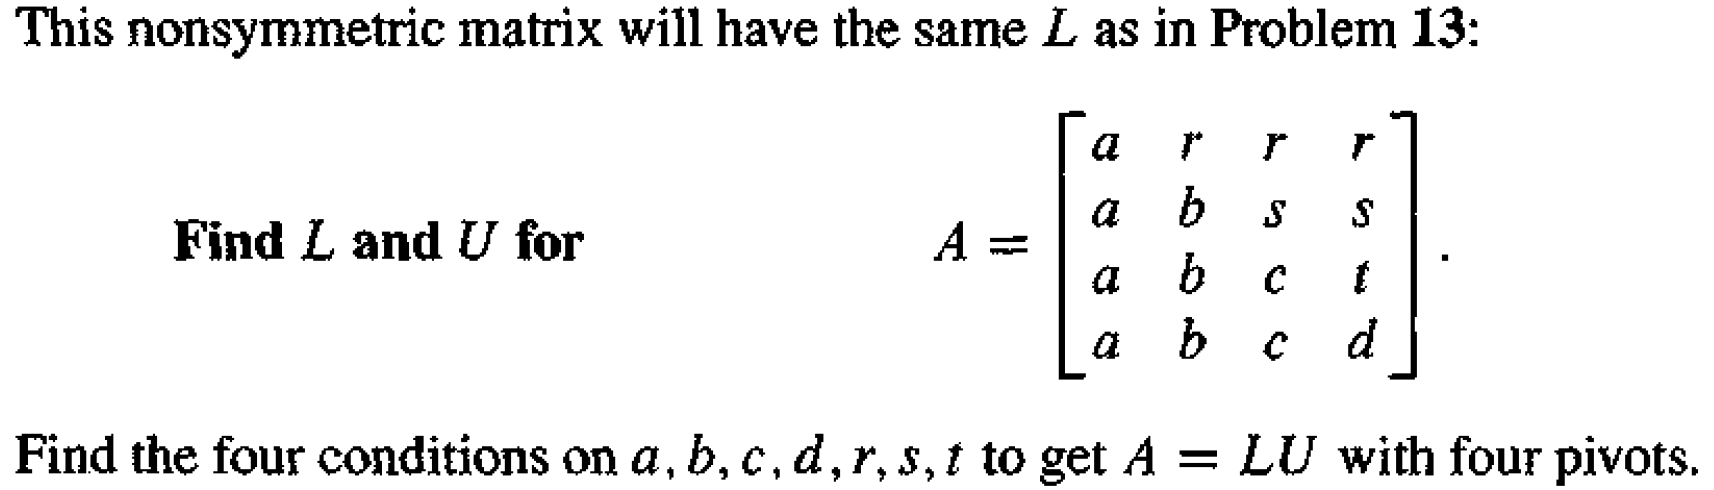
\includegraphics[height=3cm,width=1\textwidth,keepaspectratio]{2.png}
        % \caption{caption_name}
        \label{fig:2.png}
    \end{figure}
    \uncover<2->{
        \alert{\Large Answer}
        \begin{figure}[H]
            \centering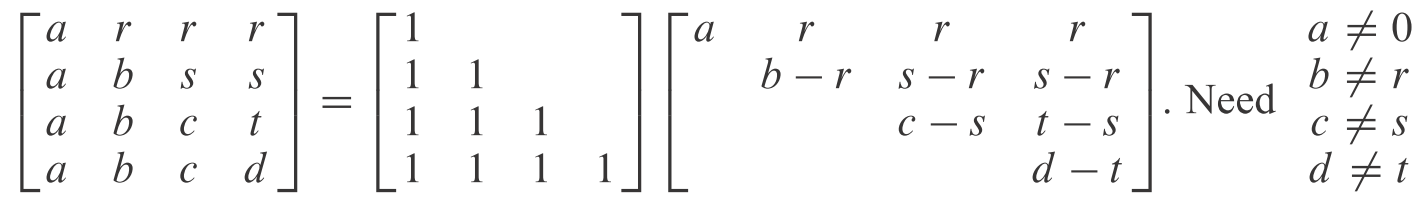
\includegraphics[height=3cm,width=1\textwidth,keepaspectratio]{2ans.png}
            % \caption{caption_name}
            \label{fig:2ans.png}
        \end{figure}
    }
\end{frame}

\begin{frame}[t]{Task 3}
    \framesubtitle{}
    \begin{figure}[H]
        \centering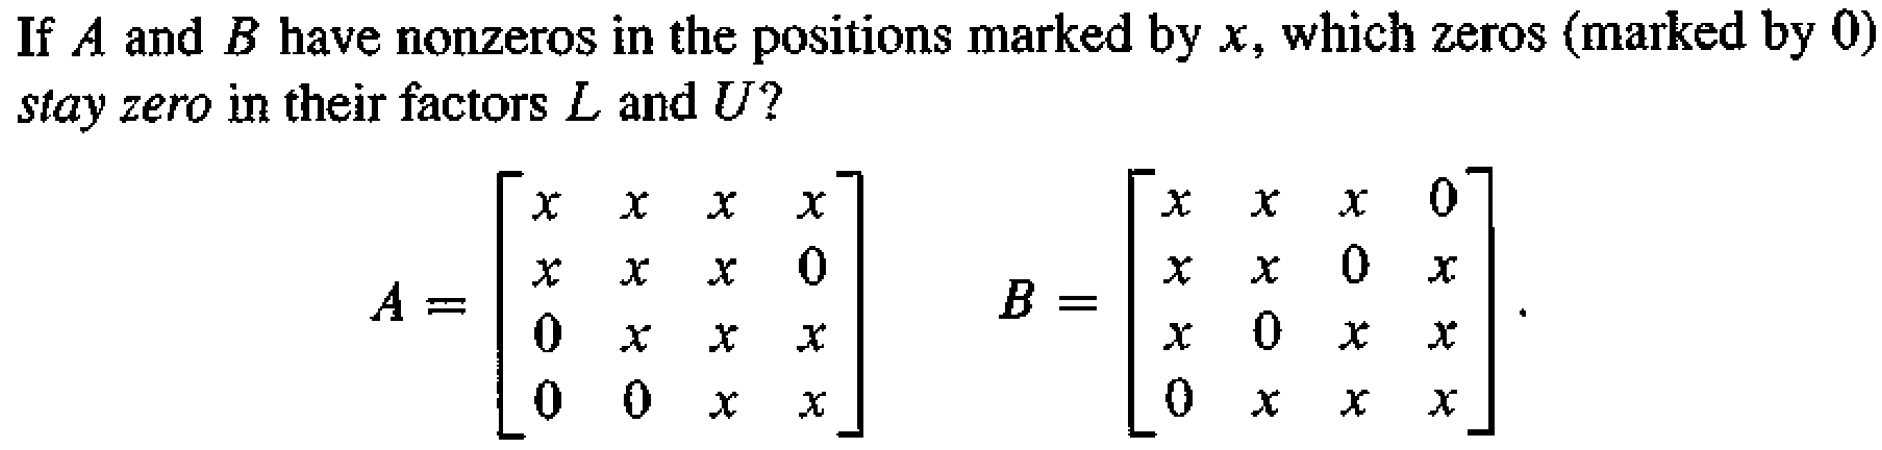
\includegraphics[height=3cm,width=1\textwidth,keepaspectratio]{3.png}
        % \caption{caption_name}
        \label{fig:3.png}
    \end{figure}
    \uncover<2->{
        \alert{\Large Answer}
        \begin{figure}[H]
            \centering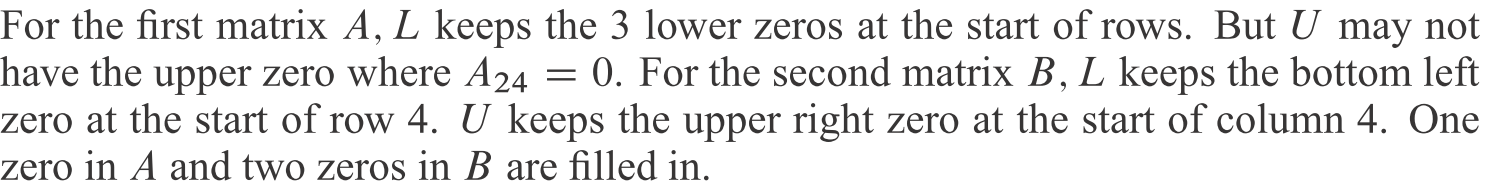
\includegraphics[height=3cm,width=1\textwidth,keepaspectratio]{3ans.png}
            % \caption{caption_name}
            \label{fig:3ans.png}
        \end{figure}
    }
\end{frame}

\begin{frame}[t]{Reference material}
    \framesubtitle{}
    \Large
    \begin{itemize}
        \item \href{https://ocw.mit.edu/courses/mathematics/18-06-linear-algebra-spring-2010/video-lectures/lecture-4-factorization-into-a-lu/}{Lecture 4 MIT course}
        \item \textit{"Linear Algebra and Applications", pdf pages 46--86 }
    \end{itemize}
\end{frame}

\fbckg{fibeamer/figs/last_page.png}
\frame[plain]{}

\end{document}